% LTeX: enabled=false

\documentclass{article}
\usepackage{tikz}
\usetikzlibrary{patterns,decorations.pathmorphing,positioning, shapes.multipart, calc,arrows, shapes.geometric}
\usepackage[dvipsnames]{xcolor}

\begin{document}

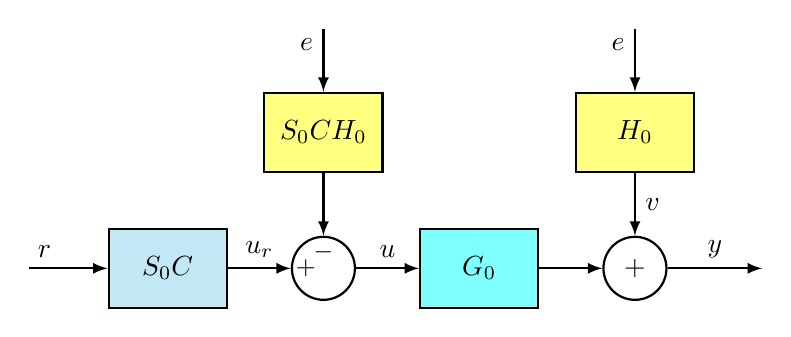
\begin{tikzpicture}[circ/.style = {draw, circle, minimum size=8mm, inner sep=0pt}, thick ]


% S0C
\node[draw, fill=SkyBlue!50, minimum width=15mm, minimum height=10mm ] (S0C) at (0,0) {$S_0 C$};
%--- G0 -> sum_v ---
\draw[-latex] ([xshift=-10mm]S0C.west) -- node[above, at start , xshift=2mm]{$r$} (S0C.west);

% sum_r1
\node[circ , right=8mm of S0C ]  (sum_r1) {};
\node[left=-1pt] at  (sum_r1.center){\small $+$};
\node[above=-1pt] at (sum_r1.center){\small $-$};

% G0
\node[draw, fill=Cyan!50, minimum width=15mm, minimum height=10mm , right=8mm of sum_r1 ] (G0)    {$G_0$};

% sum_v
\node[circ, , right=8mm of G0 ]  (sum_v) {$+$};

% H0
\node[draw, fill=Yellow!50, minimum width=15mm, minimum height=10mm, above=8mm of sum_v ] (H0)  {$H_0$};

\draw[-latex] (S0C) -- node[above]{$u_r$}(sum_r1);

%--- e -> H0 -> v -> sum_v --- % H0
\node[draw, fill=Yellow!50, minimum width=15mm, minimum height=10mm, above=8mm of sum_r1 ] (S0CH0)  {$S_0 C H_0$};
\draw[-latex] ([yshift=8mm]S0CH0.north) node[left,yshift=-2mm]{$e$} -- (S0CH0);
\draw[-latex] (S0CH0) -- node[right]{} (sum_r1);

%--- sum_r1 -> G0 ---
\draw[-latex] (sum_r1) -- node[above]{$u$} (G0);

%--- G0 -> sum_v ---
\draw[-latex] (G0) -- (sum_v);

%--- e -> H0 -> v -> sum_v ---
\draw[-latex] ([yshift=8mm]H0.north) node[left,yshift=-2mm]{$e$} -- (H0);
\draw[-latex] (H0) -- node[right]{$v$} (sum_v);

%--- sum_v -> y output ---
\draw[-latex] (sum_v) -- node[above]{$y$} ([xshift=12mm] sum_v.east);


\end{tikzpicture}
\end{document}
